\documentclass[a4paper,titlepage,11pt,twosides,floatssmall]{mwrep}
\usepackage[left=2.5cm,right=2.5cm,top=2.5cm,bottom=2.5cm]{geometry}
\usepackage[OT1]{fontenc}
\usepackage{polski}
\usepackage{amsmath}
\usepackage{amsfonts}
\usepackage{amssymb}
\usepackage{graphicx}
\usepackage{url}
\usepackage{tikz}
\usetikzlibrary{arrows,calc,decorations.markings,math,arrows.meta}
\usepackage{rotating}
\usepackage[percent]{overpic}
\usepackage[cp1250]{inputenc}
\usepackage{xcolor}
\usepackage{pgfplots}
\usetikzlibrary{pgfplots.groupplots}
\usepackage{listings}
\usepackage{matlab-prettifier}
\usepackage{siunitx}
\usepackage[section]{placeins}
\definecolor{szary}{rgb}{0.95,0.95,0.95}
\sisetup{detect-weight,exponent-product=\cdot,output-decimal-marker={,},per-mode=symbol,binary-units=true,range-phrase={-},range-units=single}
\SendSettingsToPgf

%konfiguracje pakietu listings
\lstset{
	backgroundcolor=\color{szary},
	frame=single,
	breaklines=true,
}
\lstdefinestyle{customlatex}{
	basicstyle=\footnotesize\ttfamily,
	%basicstyle=\small\ttfamily,
}
\lstdefinestyle{customc}{
	breaklines=true,
	frame=tb,
	language=C,
	xleftmargin=0pt,
	showstringspaces=false,
	basicstyle=\small\ttfamily,
	keywordstyle=\bfseries\color{green!40!black},
	commentstyle=\itshape\color{purple!40!black},
	identifierstyle=\color{blue},
	stringstyle=\color{orange},
}
\lstdefinestyle{custommatlab}{
	captionpos=t,
	breaklines=true,
	frame=tb,
	xleftmargin=0pt,
	language=matlab,
	showstringspaces=false,
	%basicstyle=\footnotesize\ttfamily,
	basicstyle=\scriptsize\ttfamily,
	keywordstyle=\bfseries\color{green!40!black},
	commentstyle=\itshape\color{purple!40!black},
	identifierstyle=\color{blue},
	stringstyle=\color{orange},
}

%wymiar tekstu (bez �ywej paginy)
\textwidth 160mm \textheight 247mm

%ustawienia pakietu pgfplots
\pgfplotsset{
tick label style={font=\scriptsize},
label style={font=\small},
legend style={font=\small},
title style={font=\small}
}

\def\figurename{Rys.}
\def\tablename{Tab.}

%konfiguracja liczby p�ywaj�cych element�w
\setcounter{topnumber}{0}%2
\setcounter{bottomnumber}{3}%1
\setcounter{totalnumber}{5}%3
\renewcommand{\textfraction}{0.01}%0.2
\renewcommand{\topfraction}{0.95}%0.7
\renewcommand{\bottomfraction}{0.95}%0.3
\renewcommand{\floatpagefraction}{0.35}%0.5

\begin{document}
\frenchspacing
\pagestyle{uheadings}

%strona tytu�owa
\title{\bf Sprawozdanie z laboratorium nr 1\vskip 0.1cm}
\author{Sobolewski Konrad, R�a�ski Antoni, Gie�dowski Daniel }
\date{2017}

\makeatletter
\renewcommand{\maketitle}{\begin{titlepage}
\begin{center}{\LARGE {\bf
Wydzia� Elektroniki i Technik Informacyjnych}}\\
\vspace{0.4cm}
{\LARGE {\bf Politechnika Warszawska}}\\
\vspace{0.3cm}
\end{center}
\vspace{5cm}
\begin{center}
{\bf \LARGE Projektowanie uk�ad�w sterowania\\ (projekt grupowy) \vskip 0.1cm}
\end{center}
\vspace{1cm}
\begin{center}
{\bf \LARGE \@title}
\end{center}
\vspace{2cm}
\begin{center}
{\bf \Large \@author \par}
\end{center}
\vspace*{\stretch{6}}
\begin{center}
\bf{\large{Warszawa, \@date\vskip 0.1cm}}
\end{center}
\end{titlepage}
}
\makeatother

\maketitle

\tableofcontents
\chapter{Laboratorium: Opis obiektu}
\label{sec:opis}
Obiektem u�ywanym na laboratorium by�o stanowisko grzej�co-ch�odz�ce przedstawione schematycznie na poni�szym rysunku \ref{stanowisko}. Stanowisko sk�ada si� z 4 wentylator�w (W), 2 grza�ek (G), 5 czujnik�w temperatury (T), pomiaru pr�du (P1) oraz napi�cia (P2). Nie korzystali�my jednak w tym �wiczeniu ze wszystkich element�w stanowiska. Przez ca�y czas trwania �wiczenia uruchomiony by� tylko wentylatoray W1, kt�ry ustawiony na sta�e  $50\%$ mocy symulowa�y sta�e niemierzalne zak��cenie. Symulowany by� obiekt o jednym wej�ciu i jednym wyj�ciu - sterowaniem naszego obiektu by�a grza�ka G1. Jako wyj�cie zosta� przyj�ty czujnik temperatury T1. Nie odczytywali�my warto�ci z pozosta�ych czujnik�w; nie by�y one istotne dla naszego eksperymentu. Ze wzgl�du na to, �e mierzonym medium by�a temperatura, obiekt by� nara�ony na r�nego rodzaju szumy i zak��cenia. Jego po�o�enie tak�e nie sprzyja�o dok�adnym pomiarom (otwarte drzwi). Z tych powod�w pomiary z niego otrzymane mog�y zawiera� odchylenia od warto�ci w�a�ciwej.

\begin{figure}[tb]
\centering
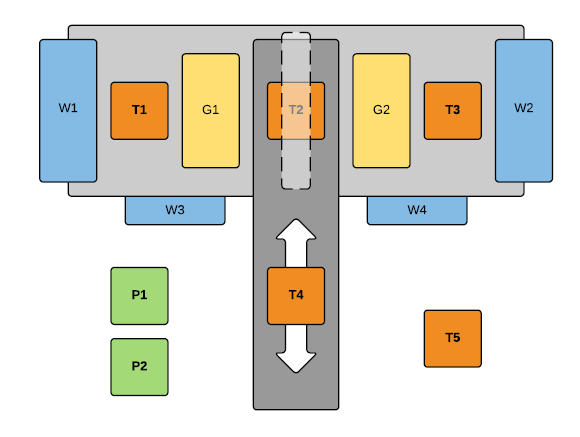
\includegraphics{wykresy/stanowisko.png}
\caption{Schemat stanowiska grzej�co-ch�odz�cego}
\label{stanowisko}
\end{figure}
\chapter{Zadanie 1: Punkt pracy}
Pierwszym poleceniem by�o okre�lenie warto�ci wyj�cia obiektu $Y_{pp}$ (pomiaru $T1$) w punkcie pracy $U_{pp} = 36$. Osi�gn�li�my j� ustawiaj�c warto�� sterowania (moc grzania grza�ki $G1$) na $U_{pp}$ i odczekuj�c znaczn� ilo�� czasu (powy�ej 5 minut). Jak wida� na wykresie \ref{pp}, wyj�cie ustabilizowa�o si� w okolicy 35 stopni Celcjusza. Jendak�e, z powodu narastaj�cej temperatury w ci�gu zaj��, punkt pracy zmienia� si�, nawet o ponad stopie� w g�r�, co b�dzie widoczne w nast�pnych zadaniach.


\begin{figure}[tb]
	\centering
	\begin{tikzpicture}
	\begin{axis}[
	legend pos=south east,
	width=0.9\textwidth,
	xmin=0,xmax=300,ymin=25,ymax=37,
	xlabel={$k$},
	ylabel={$S(k)$},
	xtick={0,50,100,150,200,250,300},
	ytick={25,26,27,28,29,30,31,32,33,34,35,36,37},
	y tick label style={/pgf/number format/1000 sep=},
	]
	\addplot[blue,semithick] file {wykresy/lab1U.txt};
	\addplot[red,semithick] file {wykresy/lab1Y.txt};
	
	\legend{$U$,$Y$}
	\end{axis}
	\end{tikzpicture}
	\caption{Zachowanie obiektu w punkcie pracy, $U_{pp}=\num{36}$}
	\label{pp}
\end{figure}
\FloatBarrier
\chapter{Zadanie 2: Odpowiedzi skokowe}
\section{Odpowiedzi skokowe}

W tej cz�ci projektu nale�a�o wyznaczy� symulacyjnie odpowiedzi skokowe (rys. \ref{odpskok}). Eksperyment zak�ada�, i� obiekt b�dzie na pocz�tku w punkcie pracy, a nast�pnie w chwili $k=15$ zostanie wykonany skok jednostkowy. 
\begin{figure}[tb]
	\centering
	\begin{tikzpicture}
	\begin{axis}[
	width=0.9\textwidth,
	height=0.3\textheight,
	xmin=0,xmax=150,ymin=-1,ymax=1,
	xlabel={$k$},
	ylabel={$U$},
	xtick={0,50,100,150},
	ytick={-1,-0.5,0,0.5,1},
	]
	\addplot[blue,semithick] file {wykresy/zad2/z2_u1.txt};
	\addplot[red,semithick] file {wykresy/zad2/z2_u4.txt};
	\addplot[green,semithick] file {wykresy/zad2/z2_u7.txt};
	\addplot[yellow,semithick] file {wykresy/zad2/z2_u10.txt};
	\addplot[brown,semithick] file {wykresy/zad2/z2_u13.txt};
	\addplot[orange,semithick] file {wykresy/zad2/z2_u16.txt};
	\addplot[magenta,semithick] file {wykresy/zad2/z2_u19.txt};
	\end{axis}
	\end{tikzpicture}
	\caption{Sterowanie}
	\label{uskok}
\end{figure}

\begin{figure}[tb]
	\centering
	\begin{tikzpicture}
	\begin{axis}[
	width=0.9\textwidth,
	height=0.3\textheight,
	xmin=0,xmax=200,ymin=-0.5,ymax=6,
	xlabel={$k$},
	ylabel={$Y$},
	xtick={0,50,100,150,200},
	ytick={-0.5,0,0.5,1,1.5,2,2.5,3,3.5,4,4.5,5,5.5,6},
	]
	\addplot[blue,semithick] file {wykresy/zad2/z2_y1.txt};
	\addplot[red,semithick] file {wykresy/zad2/z2_y4.txt};
	\addplot[green,semithick] file {wykresy/zad2/z2_y7.txt};
	\addplot[yellow,semithick] file {wykresy/zad2/z2_y10.txt};
	\addplot[brown,semithick] file {wykresy/zad2/z2_y13.txt};
	\addplot[orange,semithick] file {wykresy/zad2/z2_y16.txt};
	\addplot[magenta,semithick] file {wykresy/zad2/z2_y19.txt};
	\end{axis}
	\end{tikzpicture}
	\caption{Wyj�cie}
	\label{yskok}
\end{figure}


\section{Charakterystyka statyczna}
Poni�ej zosta�a zaprezentowana charakterystyka statyczna procesu $y(u)$ (rys. \ref{stat}).
Na podstawie zawartego wykresu mo�na wywnioskowa�, �e w�a�ciwo�ci statyczne procesu s� nieliniowe. 

\begin{figure}[tb]
	\centering
	\begin{tikzpicture}
	\begin{axis}[
	width=0.9\textwidth,
	height=0.5\textheight,
	xmin=-1,xmax=1,ymin=-0.5,ymax=6,
	xlabel={$U$},
	ylabel={$Y$},
	xtick={-1,-0.8,-0.6,-0.4,-0.2,0,0.2,0.4,0.6,0.8,1},
	ytick={-0.5,0,0.5,1,1.5,2,2.5,3,3.5,4,4.5,5,5.5,6},
	]
	\addplot[blue,semithick] file {wykresy/zad2/z2_stat.txt};
	\end{axis}
	\end{tikzpicture}
	\caption{Charakterystyka statyczna}
	\label{stat}
\end{figure}

\section{Charakterystyka dynamiczna}
Charakterystyka dynamiczna zosta�a wyznaczona zale�nie od wielko�ci skoku sterowania. Zmierzone zosta�o, po ilu krokach od momentu skoku r�nica warto�ci wyj�� obiektu i punktu pracy $Y_{pp}$ wynosi�a powy�ej $90\%$ ca�kowitego skoku warto�ci  wyj�� obiektu $Y(k)$. Z otrzymanych danych wynika, �e charakterystyka dynamiczna jest nieliniowa (rys. \ref{dynamiczna}).
\begin{figure}[tb]
	\centering
	\begin{tikzpicture}
	\begin{axis}[
	width=0.9\textwidth,
	height=0.5\textheight,
	xmin=-1,xmax=1,ymin=0,ymax=18,
	xlabel={$U$},
	ylabel={$Y$},
	xtick={-1,-0.8,-0.6,-0.4,-0.2,0,0.2,0.4,0.6,0.8,1},
	ytick={0,2,4,6,8,10,12,14,16,18},
	]
	\addplot[blue,semithick] file {wykresy/zad2/z2_dyn.txt};
	\end{axis}
	\end{tikzpicture}
	\caption{Charakterystyka dynamiczna}
	\label{dynamiczna}
\end{figure}
\chapter{Laboratorium: Zadanie 3: Znormalizowane odpowiedzi skokowe}
Kolejnym poleceniem by�o wyznaczy� znormalizowane odpowiedzi skokowe (takie jakie wymagane s� do algorytmu DMC) i zaproksymowa� je, u�ywaj�c w tym celu cz�onu inercyjnego drugiego rz�du z op�nieniem. Cz�on posiada 4 parametry: $T_1$, $T_2$, $K$ (dalej oznaczane jako $K_p$) i $T_d$ (w dalszej cz�ci sprawozdania oznaczane jako $TD$). Nazwy zosta�y zmienione, by nie myli� ich z parametrami algorytmu PID. Cz�on jest opisany wzorami powsta�ymi po przekszta�ceniu jego transmitancji:
\begin{equation}
\alpha_1=e^{-\frac{1}{T_1}}
\end{equation}
\begin{equation}
\alpha_2=e^{-\frac{1}{T_2}}
\end{equation}
\begin{equation}
a_1=-\alpha_1-\alpha_2
\end{equation}
\begin{equation}
a_1=\alpha_1\alpha_2
\end{equation}
\begin{equation}
b_1=\frac{K_p}{T_1-T_2}[T_1(1-\alpha_1)-T_2(1-\alpha_2)]
\end{equation}
\begin{equation}
b_1=\frac{K_p}{T_1-T_2}[\alpha_1T_2(1-\alpha_2)-\alpha_2T_1(1-\alpha_1)]
\end{equation}
\begin{equation}
y(k)=b_1u(k-TD-1)+b_2u(k-TD-2)-a_1y(k-1)-a_2y(k-2)
\end{equation}
\\
W celu doboru parametr�w cz�onu wykorzystano funkcj� fmincon. Jako pocz�tkowe warto�ci dobieranych parametr�w wybrali�my $[11,10,1,10]$, 11 i 10 dla $T_1$ i $T_2$, aby nie by�y takie same, 1 dla $K_p$, bo przy dotychczas zebranych przebiegach nie spodziewali�my si� du�ego wzmocnienia dla tego obiektu i 10 dla $TD$, bo z obserwacji wynika, �e op�nienie obiektu jest bliskie tej warto�ci. Od do�u ograniczyli�my wszystkie parametry zerami. Od g�ry ograniczyli�my je warto�ciami $[1000,1000,10,30]$, tak, by ka�dy parametr mia� przedzia� dostosowany do swoich potrzeb (du�e zmiany dla $T_1$ i $T_2$, ma�e zmiany dla $K_p$, $TD$ s�dz�c po wykresach nie powinno przekroczy� 30). 
\section{Wyb�r odpowiedzi skokowej}
�wiadomi faktu, �e dla obiektu nieliniowego, jakim jest stanowisko grzewcze, liniowy algotyrm DMC nie b�dzie dzia�a� optymalnie, postanowili�my przyj�� tak� odpowied�, �eby regulowa� poprawnie przynajmniej w dolnej cz�ci zakresu temperatur i cz�ciowo w jego g�rnej. Dlatego jako odpowied� do znormalizowania wybrali�my t� dla skoku o $dU = 15$, jako �e zawiera w sobie ca�y dolny zakres oraz niewielk� cz�� g�rnego. W wyniku normalizacji przekszta�cili�my j� do odpowiedzi jak� mieliby�my po skoku jednostkowym (odj�li�my od ka�dej zebranej pr�bki warto�� w punkcie pracy dla danego wyj�cia i podzielili�my otrzymane warto�ci przez skok). Nast�pnie po wykonaniu aproksymacji otrzymali�my parametry cz�onu r�wne $T_1 = 71,0271$, $T_2 = 5,2254$, $K_p = 0,3935$ i $Td = 13$ przy b��dzie optymalizacji $e = 0,0038$. Znormalizowan� odpowied� i jej aproksymacj� przedstawili�my na poni�szym wykresie \ref{norm_skoky}.

\begin{figure}[tb]
\centering
\begin{tikzpicture}
\begin{axis}[
width=0.9\textwidth,
xmin=0,xmax=300,ymin=0,ymax = 0.45,
xlabel={$k$},
ylabel={$S(k)$},
xtick={0,50,100,150,200,250,300,350},
ytick={0,0.1,0.2,0.3,0.4,0.5,0.6},
y tick label style={/pgf/number format/1000 sep=},
legend pos=south east,
]
\addplot[blue,semithick] file {wykresy/lab3_15.txt}; 
\addplot[orange,semithick] file{wykresy/aprskok15.txt};

\legend{odpowied� skokowa,aproksymacja}
\end{axis}
\end{tikzpicture}
\caption{Wykres znormalizowanej odpowiedzi skokowej i jej aproksymacji}
\label{norm_skoky}
\end{figure}
\chapter{Zadanie 4: Algorytmy PID i DMC}
W projektowanych regulatorach $PID$ i $DMC$ zosta�y zastosowane nast�puj�ce ograniczenia:
\begin{equation}
\triangle U^{\mathrm{max}} = 0,05
\label{dUmax}
\end{equation}

\begin{equation}
\begin{split}
\textrm{jezeli  }
\triangle U(k) >
\triangle U^{\mathrm{max}}
\textrm{   to   }
\triangle U(k) = 
\triangle U^{\mathrm{max}} \\
\textrm{jezeli  }
\triangle U(k) < -
\triangle U^{\mathrm{max}}
\textrm{   to   }
\triangle U(k) = -
\triangle U^{\mathrm{max}}
\label{ogr1}
\end{split}
\end{equation}

\begin{equation}
\begin{split}
\textrm{jezeli  }
U(k) > U^{\mathrm{max}}
\textrm{   to   }
U(k) =  U^{\mathrm{max}} \\
\textrm{jezeli  }
U(k) < U^{\mathrm{min}}
\textrm{   to   }
U(k) =  U^{\mathrm{min}}
\label{ogr2}
\end{split}
\end{equation}


\section{Cyfrowy algorytm PID}

W projekcie zosta� wykorzystany regulator cyfrowy $PID$, kt�rego parametry s� opisane poni�szymi wzorami, gdzie 
$K$ - wzmocnienie cz�onu P , $T_p$ - czas pr�bkowania, $T_i$ - czas zdwojenia cz�onu ca�kuj�cego $I$, $T_d$ - czas wyprzedzenia cz�onu r�niczkuj�cego $D$. 
\begin{equation}
r_0=K*(1+T_p/(2*T_i)+T_d/T_p) 
\label{r0}
\end{equation}

\begin{equation}
r_1=K*(T_p/(2*T_i)-2*T_d/T_p-1)
\label{r1}
\end{equation}

\begin{equation}
r_2=K*T_d/T_p
\label{r2}
\end{equation}
W ka�dej iteracji p�tli sterowania jest obliczany uchyb wyj�cia obiektu od warto�� zadanej jego wyj�cia.
\begin{equation}
e(k) = Y^{\mathrm{zad}}(k) - Y(k);
\label{uchyb}
\end{equation}
Sterowanie regulatora zostaje wyliczone na bie��c� chwile przy u�yciu wzoru:
\begin{equation}
U(k) = r_2*e(k-2) + r_1*e(k-1) + r_0*e(k) + U(k-1);
\label{Uk}
\end{equation}

\section{Analityczny algorytm DMC}
Do oblicze� wykorzystujemy nast�puj�ce wzory:
\begin{equation}
\boldsymbol{Y}^{\mathrm{zad}}(k)=\left[
\begin{array}{c}
Y^{\mathrm{zad}}(k)\\
\vdots\\
Y^{\mathrm{zad}}(k)
\end{array}
\right]_{\mathrm{Nx1}}
\label{yzadm}
\end{equation}

\begin{equation}
\boldsymbol{Y}(k)=\left[
\begin{array}{c}
y(k)\\
\vdots\\
y(k)
\end{array}
\right]_{\mathrm{Nx1}}
\label{ym}
\end{equation}

\begin{equation}
\triangle\boldsymbol{U}(k)=\left[
\begin{array}{c}
\triangle u(k|k)\\
\vdots\\
\triangle u(k+N_u -1 |k)
\end{array}
\right]_{\mathrm{N_ux1}}
\label{dUm}
\end{equation}

\begin{equation}
\triangle\boldsymbol{U^P}(k)=\left[
\begin{array}{c}
\triangle u(k-1)\\
\vdots\\
\triangle u(k-(D-1))
\end{array}
\right]_{\mathrm{(D-1)x1}}
\label{dUPm}
\end{equation}

\begin{equation}
\boldsymbol{M}=\left[
\begin{array}
{cccc}
s_{1} & 0 & \ldots & 0\\
s_{2} & s_{1} & \ldots & 0\\
\vdots & \vdots & \ddots & \vdots\\
s_{N} & s_{N-1} & \ldots &  s_{N-N_{\mathrm{u}}+1}
\end{array}
\right]_{\mathrm{NxN_u}}
\label{Mm}
\end{equation}

\begin{equation}
\boldsymbol{M^P}=\left[
\begin{array}
{cccc}
s_{2}-s_{1} & s_{3}-s_{2} & \ldots & s_{D}-s_{D-1}\\
s_{3}-s_{1} & s_{4}-s_{2} & \ldots & s_{D+1}-s_{D-1}\\
\vdots & \vdots & \ddots & \vdots\\
s_{N+1}-s_{1} & s_{N+2}-s_{2} & \ldots &  s_{N+D-1}-S_{D-1}
\end{array}
\right]_{\mathrm{NxD-1}}
\label{MPm}
\end{equation}

\begin{equation}
Y^0(k)=Y(k)+M^P
\triangle U^P(k)
\label{Y0}
\end{equation}

\begin{equation}
K=(M^TM+\lambda*I)^{-1}M^T
\label{K}
\end{equation}

\begin{equation}
\triangle U(k)=K(Y^{zad}(k)-Y^0(k))
\label{dU1}
\end{equation}

W naszej regulacji potrzebujemy wyznaczy� tylko pierwszy element macierzy $\triangle U(k)$ czyli $\triangle u(k|k)$. W tym celu rozwijamy wz�r do postaci:

\begin{equation}
\triangle u(k|k)=k_ee(k)-k_u\triangle\boldsymbol U^P
\label{dukk}
\end{equation}

gdzie:

\begin{equation}
e(k)=Y^{zad}(k)-Y(k)
\label{e}
\end{equation}

\begin{equation}
k_e=\sum_{i=1}^N K(1,i)
\label{ke}
\end{equation}

\begin{equation}
k_u=kM^P
\label{ku}
\end{equation}

k to oznaczenie pierwszego wiersza macierzy K. Aktualne sterowanie otrzymujemy poprzez zsumowanie poprzedniego sterowania i aktualnie wyliczonego $\triangle u(k|k)$. 
\chapter{Laboratorium: Zadanie 5: Strojenie regulatora PID i DMC}
Strojenie regulataora odby�o si� na podstawie oceny regulacji dla zaproponowaej trajektorii zmian sygna��w zadanych sk�adaj�cej si� z sze�ciu skok�w. Warto�ci zadane zosta�y tak dobrane, aby za ka�dym razem by�a inna warto�� skoku.

\section{Regulator PID}

\subsection{Pocz�tkowe nastawy}
Nastawy regulatora PID zosta�y dobrane eksperymentalnie. Sugeruj�c si� nastawami otrzymanymi na poptrzednich laboratoriach, jako warto�ci pocz�tkowe przyj�li�my nastawy: $K_p = 5, T_i = 75, T_d = 1.25$. Na rys. \ref{PID1} mo�na obserwowa� prac� regulatora z takimi nastawami. Jak wida�, nie s� to nastawy optymalne; regulator jest nieskuteczny. Dla dolnego przedzia�u dzia�a lepiej, w g�rnym jest zdecydowanie zbyt s�aby. B��d wyj�cia $Y$ wyni�s�: $E = 5042,6750$.



\begin{figure}[tb]
	\centering
	\begin{tikzpicture}
	\begin{groupplot}[group style={group size=1 by 2,vertical sep={2 cm}},
	width=0.9\textwidth,height=0.5\textwidth]
	\nextgroupplot
	[
	xmin=0,xmax=1210,ymin=-5,ymax=105,
	xlabel={$k$},
	ylabel={$U(k)$},
	xtick={0,100,200,300,400,500,600,700,800,900,1000,1100,1200},
	ytick={0,10,20,30,40,50,60,70,80,90,100},
	y tick label style={/pgf/number format/1000 sep=},
	legend pos=south east,
	]
	\addplot[blue,semithick] file {wykresy/lab4pidU_5.0000_75.0000_1.2500.txt};
	\nextgroupplot
	[
	xmin=0,xmax=1210,ymin=36,ymax=46,
	xlabel={$k$},
	ylabel={$Y(k)$},
	xtick={0,100,200,300,400,500,600,700,800,900,1000,1100,1200},
	ytick={36,37,38,39,40,41,42,43,44,45,46},
	y tick label style={/pgf/number format/1000 sep=},
	legend pos=north east,
	]
	\addplot[red,semithick] file{wykresy/lab4pidY_5.0000_75.0000_1.2500.txt}; 
	\addplot[orange,semithick,densely dashed] file{wykresy/lab4Yzad.txt}; 
	\legend{$Y$,$Y^{zad}$,$Y_2$,}
	\end{groupplot}
	\end{tikzpicture}
	\caption{Dzia�anie algorytmu PID przy pocz�tkowych nastawach  $K_p = 5, T_i = 75, T_d = 1.25$} 
	\label{PID1}
\end{figure}
\FloatBarrier

\subsection{Korygowanie  nastaw}
Aby poprawi� osi�gi regualtora w przedziale wy�szych warto�ci temperatury, a tak�e poprawi� zbyt wolna regulacj� temperatury widoczn� w pobli�u $k = 1100$, postanowili�my zwi�kszy� wp�yw cz�onu ca�kuj�cego, obni�aj�c $T_i$ do warto�ci $T_i = 65$ oraz zmniejszy� wp�yw cz�onu r�niczkuj�cego - nowe  $T_d = 1$. Wzmocnienie nie by�o zmieniane, gdy� obawiali�my si� pogorszenia regulacji w dolnym przedziale temperatur. Tak wi�c nowe nastawy to: $K_p = 5, T_i = 65, T_d = 1$. Dla takich nastaw osi�gn�li�my przebiegi jak na \ref{PID2}. 


\begin{figure}[tb]
	\centering
	\begin{tikzpicture}
	\begin{groupplot}[group style={group size=1 by 2,vertical sep={2 cm}},
	width=0.9\textwidth,height=0.6\textwidth]
	\nextgroupplot
	[
	xmin=0,xmax=1210,ymin=-5,ymax=105,
	xlabel={$k$},
	ylabel={$U(k)$},
	xtick={0,100,200,300,400,500,600,700,800,900,1000,1100,1200},
	ytick={0,10,20,30,40,50,60,70,80,90,100},
	y tick label style={/pgf/number format/1000 sep=},
	legend pos=south east,
	]
	\addplot[blue,semithick] file {wykresy/lab4pidU_5.0000_65.0000_1.0000.txt};
	\nextgroupplot
	[
	xmin=0,xmax=1210,ymin=36,ymax=46,
	xlabel={$k$},
	ylabel={$Y(k)$},
	xtick={0,100,200,300,400,500,600,700,800,900,1000,1100,1200},
	ytick={36,37,38,39,40,41,42,43,44,45,46},
	y tick label style={/pgf/number format/1000 sep=},
	legend pos=north east,
	]
	\addplot[red,semithick] file{wykresy/lab4pidY_5.0000_65.0000_1.0000.txt}; 
	\addplot[orange,semithick,densely dashed] file{wykresy/lab4Yzad.txt}; 
	\legend{$Y$,$Y^{zad}$,$Y_2$,}
	\end{groupplot}
	\end{tikzpicture}
	\caption{Dzia�anie algorytmu PID przy zmodyfikowanych nastawach  $K_p = 4, T_i = 65, T_d = 1$} 
	\label{PID2}
\end{figure}
\FloatBarrier

Otrzymany regulator zapewnia lepsz� jako�� regulacji - b��d wyj�cia $Y$ si� zmniejszy� i wyni�s�: $E = 42436,6750$. Chocia� wy�sza ca�ka pogorszy�a regulacj� w dolnym zakresie regulacji, to regulator osi�ga teraz szybciej warto�� zadan� tak�e w wy�szym zakresie. Obserwujemy jednak wci�� uchyb ustalony przy skoku z ok. 44 stopni na ok. 37 stopnie.

\section{Laboratorium: Regulator DMC}

Nast�pnie pr�bowali�my zastosowa� do nieliniowego obiektu, jakim by�o stanowisko grzewcze, regulacj� DMC. Do u�ycia w modelu wybrali�my odpowied� skokow� przy $dU = 15$.

\subsection{Pocz�tkowe nastawy}
Nastawy regulatora DMC zosta�y dobrane eksperymentalnie. Jako warto�ci pocz�tkowe przyj�li�my nastawy $N = 300$, $Nu = 300$, $\lambda = 0.5$. Warto�� $300$ wynika z obserwacji obiektu - bezpiecznie za�o�yli�my, �e tyle wynosi jego horyzont dynamiki. Obiekt ten nie jest wra�liwy na nag�e zmiany sterowa� a tak�e na poprzednich laboratoriach lambda przyjmowa�a ma�e warto�ci - dlatego zdecydowali�my na pocz�tek przyj�� $\lambda = 0.5$. Na rys. \ref{DMC_begin} mo�na obserwowa� prac� regulatora z takimi nastawami. Regulator dzia�a poprawnie, z pewno�ci� lepiej ni� regulator PID; zar�wno przebiegi wyj�cia s� bli�sze warto�ci zadanej jak i sterowania s� �agodniejsze. Nie s� to jednak nastawy optymalne; regulator powienien dzia�a� szybciej w wy�szym zakresie temperatur. B��d wyj�cia, znacz�co mniejszy ni� dla regulatoar PID wyni�s� $E = 3513,38$.
	\begin{figure}
	\centering
	\begin{tikzpicture}
	\begin{groupplot}[group style={group size=1 by 2,vertical sep={2 cm}},
	width=0.9\textwidth,height=0.6\textwidth]
	\nextgroupplot
	[
	xmin=0,xmax=1210,ymin=-5,ymax=105,
	xlabel={$k$},
	ylabel={$U(k)$},
	xtick={0,100,200,300,400,500,600,700,800,900,1000,1100,1200},
	ytick={0,10,20,30,40,50,60,70,80,90,100},
	y tick label style={/pgf/number format/1000 sep=},
	legend pos=south east,
	]
	\addplot[blue,semithick] file {wykresy/lab4dmcU_300_0.5000.txt};
	\nextgroupplot
	[
	xmin=0,xmax=1210,ymin=36,ymax=46,
	xlabel={$k$},
	ylabel={$Y(k)$},
	xtick={0,100,200,300,400,500,600,700,800,900,1000,1100,1200},
	ytick={36,37,38,39,40,41,42,43,44,45,46},
	y tick label style={/pgf/number format/1000 sep=},
	legend pos=north east,
	]
	\addplot[red,semithick] file {wykresy/lab4dmcY_300_0.5000.txt};
	\addplot[orange,semithick,densely dashed] file{wykresy/lab4Yzad.txt}; 
	\legend{$Y$,$Y^{zad}$}
	\end{groupplot}
	\end{tikzpicture}
	\caption{Dzia�anie algorytmu DMC przy pocz�tkowych nastawach  $N = 300$, $Nu = 300, \lambda = 0.5$} 
	\label{DMC_begin}
	\end{figure}
	\FloatBarrier

\section{Korekta parametru Nu}
Nast�pnie przyst�pili�my do zmian nastaw: parametr N pozostawili�my bez zmian, jako �e zar�wno teoria jak i nasza praktyka wskazywa�y, �e jego zmniejszanie, je�li w og�le, prowadzi�o do minimalnych zysk�w w jako�ci sterowania. Gdyby by� to obiekt szybszy lub dzia�aj�cy w wymagaj�cym �rodowisku, mo�na by rozwa�y� skr�cenie tej warto�ci w celu zmniejszenia z�o�ono�ci obliczeniowej, jednak dla okresu pr�bkowania $Tp = 1$ nie jest to konieczne. 
Wykonali�my dwukrotnie eksperyment kolejno dla warto�ci $Nu = 150$ (rys. \ref{DMC_p2}) oraz $Nu = 100$ (rys. \ref{DMC_p3}). 
B��dy w pierwszym eksperymencie osi�gn�y warto�ci: dla $Y_1$: $E_1 = 454,2170$, dla $Y_2$: $E_2 = 439,2227$. ��czny: $E = 893,4397$.

Natomiast za drugim razem: dla $Y_1$: $E_1 = 375,6482$, dla $Y_2$: $E_2 = 431,5992$. ��czny: $E = 807,2474$.


\section{Korekta parametru $\lambda$}
Jako ostatni zmieniony zosta� parametr $\lambda$.
W celu poprawy szybko�ci sterowania zmiejszyli�my jego warto�� o po�ow� (rys. \ref{DMC_lambda}). 
Finalnie, b��dy osi�gn�y warto�ci: dla $Y_1$: $E_1 = 311,0436$, dla $Y_2$: $E_2 = 407,5791$. ��czny: $E = 718,6227$.



\section{Podsumowanie}
Tak jak nale�a�o si� spodziewa�, regulator DMC w stosunku do regulatora PID zapewnia lepsz� regulacj�. Zar�wno wska�nik jako�ci regulacji (dla DMC: $E = 718,6227$, dla PID: $E = 911,1790$) jak i wizualna ocena przebieg�w wyj�� i sterowania jednoznacznie wskazuj� algorytm DMC jako lepszy regulator obiektu grzewczego w laboratorium o dw�ch wej�ciach i dw�ch wyj�ciach.


\end{document}


